\documentclass[10pt,a4paper]{article}
\usepackage[latin1]{inputenc}
\usepackage{amsmath}
\usepackage{amsfonts}
\usepackage{amssymb}
\usepackage{graphicx}
\usepackage{pgf}
\usepackage{tikz}

\usetikzlibrary{arrows,automata}
\usepackage[latin1]{inputenc}


\begin{document}

	\begin{figure}
		\centering
		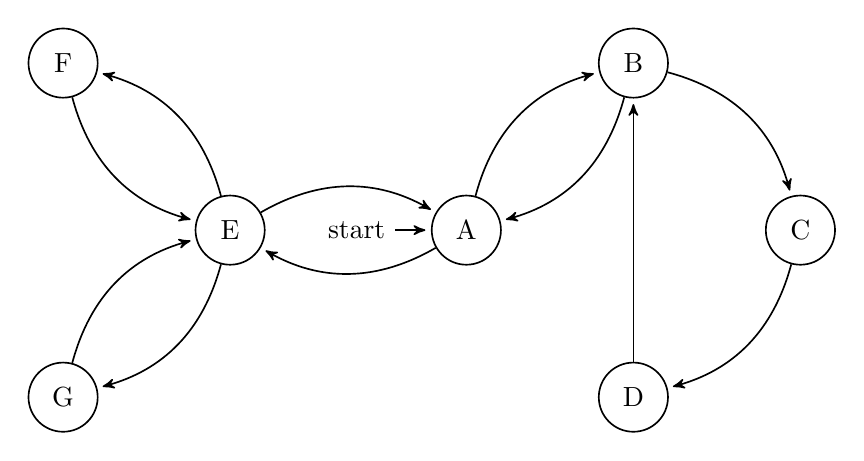
\begin{tikzpicture}[->,>=stealth',shorten >=2pt,auto,node distance=3cm,semithick]
			
			\node[state, initial] 			(A) {A};
			\node[state,above right of=A] 	(B) {B};
			\node[state,left of=A] 			(E) {E};
			\node[state,below right of=B] 	(C) {C};
			\node[state,below right of=A]   (D) {D};
			\node[state,above left of=E]    (F) {F};
			\node[state,below left of=E]    (G) {G};
			
			\path	(A)	edge[bend left]	 node { }	(E);
			\path	(E)	edge[bend left]	 node { }	(A);
			\path	(A)	edge[bend left]  node { }	(B);
			\path	(B)	edge[bend left]  node { }	(A);
			\path	(B)	edge[bend left]  node { }	(C);
			\path	(D)	edge    		 node { }	(B);
			\path	(E)	edge[bend right] node { }	(F);
			\path	(F)	edge[bend right] node { }	(E);
			\path	(E)	edge[bend left]  node { }	(G);
			\path	(G)	edge[bend left]  node { }	(E);
			\path	(C)	edge[bend left]  node { }	(D);
		\end{tikzpicture}
	\end{figure}

	STATES:
	\begin{list}{$\bullet$}{\,}
		\item A:BASE
		\item B:START
		\item C:WORK
		\item D:STOP
		\item E:TIME
		\item F:TIMEUP
		\item G:TIMEDOWN
	\end{list}
	


\end{document}